\documentclass[hyperref,german,beleg]{cgvpub}

\usepackage{fancyref}
\usepackage{acro}
\usepackage{siunitx}
\usepackage{mathtools}
\usepackage{commath}
\usepackage[ruled]{algorithm2e}
\DeclareAcronym{HAWT}{
  short = HAWT ,
  long  = Horizontal Axis Wind Turbine ,
  class = abbrev
}
\DeclareAcronym{VAWT}{
  short = VAWT ,
  long  = Vertical Axis Wind Turbine ,
  class = abbrev
}
\DeclareAcronym{DDPG}{
  short = DDPG ,
  long  = Deep Deterministic Policy Gradients ,
  class = abbrev
}
\DeclareAcronym{DQN}{
  short = DQN ,
  long  = Deep Q-Networks ,
  class = abbrev
}
\DeclareAcronym{PG}{
  short = PG ,
  long  = Policy Gradients ,
  class = abbrev
}
\DeclareAcronym{DPG}{
  short = DPG ,
  long  = Deterministic Policy Gradients ,
  class = abbrev
}
\DeclareAcronym{TD3}{
  short = TD3 ,
  long  = Twin Delayed Deep Deterministic Policy Gradients ,
  class = abbrev
}
\DeclareAcronym{REINFORCE}{
  short = REINFORCE ,
  long  = REward Increment equals Nonnegative Factor x Offset Reinforcement x Characteristic Eligibility ,
  class = abbrev
}
\DeclareAcronym{RL}{
  short = RL ,
  long  = Reinforcement Learning ,
  class = abbrev
}
\DeclareAcronym{MDP}{
  short = MDP ,
  long  = Markov Decision Process ,
  class = abbrev
}
\DeclareAcronym{PER}{
  short = PER ,
  long  = Prioritized Experience Replay ,
  class = abbrev
}
\DeclareAcronym{FMM}{
  short = FMM ,
  long  = Forward Maniac Mode ,
  class = abbrev
}
\DeclareAcronym{BMM}{
  short = BMM ,
  long  = Backward Maniac Mode ,
  class = abbrev
}
\DeclareAcronym{RFC}{
  short = RFC ,
  long  = Rainflow Counting ,
  class = abbrev
}
\DeclareAcronym{DDDDPPG}{
  short = DDPG ,
  long  = Data-augmented Double Delayed Deep Deterministic Prioritized Policy Gradients ,
  class = abbrev
}

%weitere Optionen zum Ergänzen (in eckigen Klammern):
% 
% female	weibliche Titelbezeichnung bei Diplom
% bibnum	numerische Literaturschlüssel
% final 	für Abgabe	
% lof			Abbildungsverzeichis
% lot			Tabellenverzeichnis
% noproblem	keine Aufgabenstellung
% notoc			kein Inhaltsverzeichnis
% twoside		zweiseitig
\author{Nico Westerbeck}
\title{Reinforcement-Learning Windturbine Controller}
\birthday{10. Januar 1994}
\placeofbirth{Bielefeld}
\matno{3951488}

\betreuer{Dr. Dmitrij Schlesinger}
\bibfiles{literatur}
\problem{
  \section{Background:}
  Here at the HFI Experimental fluid mechanics group, we have developed an
  open source project called QBlade. QBlade is a simulation tool used for
  testing wind turbines in the hostile environment that they normally operate.
  We normally tackle problems of aerodynamic or structural optimization but
  we have also a research focus on the development of the control systems of
  the wind turbines. We currently have a research effort looking at developing
  cluster-based controllers building on the work of Professor Bernd Noack who
  is a guest professor at our group. In the last year or so (Nair, A. G., Yeh, C.-
  A., Kaiser, E., Noack, B. R., Brunton, S. L., \& Taira, K. (2018). Cluster-based
  feedback control of turbulent post-stall separated flows. Journal of Physics
  Fluid Dynamics, (M), 1-32. Retrieved from http://arxiv.org/abs/1809.07220).
  AI projects such as openAI have enabled he rapid development of neural
  network in the field of control using reinforcement learning. The goal of this
  project is to use QBlade as a wind turbine simulator and attempt to control
  the pitch and rotor speed in a way that doesn’t cause the wind turbine to
  shatter but instead to yield energy, i.e. reward and death condition. This first
  stage of work should be considered as exploratory but will hopefully open up
  avenues of controlling active flow control elements such as flaps.

  \section{Tasks}
  The major tasks of the project are as follows:
  \begin{itemize}
    \item Build up and interface between QBlade and python the model code so that an external code can run as a controller within a QBlade simulation.
    \item Gain a rough understanding of the mechanics of wind turbines and their controllers.
    \item Research reinforcement learning methods suitable for use as a windturbine controller and perform a literature review on these approaches.
    \item Create a reinforcement learning agent which uses the Qblade interface for controllers to control a windturbine. 
      \begin{itemize}
        \item Inputs to the agent could be defined by the standartized controller input format to Nordex turbines, which consists of 39 real-valued sensor-inputs. However, initial tests can be conducted with whichever inputs are easiest to tackle. If required, further hidden state from the simulation can be exported to enrich data quality. If aiming for industrial quality, more inputs and also sensor faults could be optionally incorporated.
        \item Outputs are in a minimum version pitch angles for the 3 blades and turbine torque. Optionally the agent should be able to control active element such as flaps on the blades.
      \end{itemize}
    \item Optimize the agent to deliver maximum energy yield.
    \item Optimize under respect of certain boundary conditions (maximum pitch acceleration, maximum power, maximum blade load, blade touching the tower) and optionally other boundary conditions like long term turbine wear.
    \item If necessary for the training process, scale the simulation to run at a larger scale.
    \item Implement and attempt to get the agent to perform something close to sensible control of the wind turbine. Optionally evaluate the results against existing controllers and try to outperform them.
    \item Optionally, create a conference paper, poster or blog post etc.. on the results. 
  \end{itemize}
}


\copyrighterklaerung{Hier soll jeder Autor die von ihm eingeholten
Zustimmungen der Copyright-Besitzer angeben bzw. die in Web Press
Rooms angegebenen generellen Konditionen seiner Text- und
Bild"ubernahmen zitieren.}
\acknowledgments{At first thanks to my advisors Mattew Lennie and Dmitrij Shlezinger for their support. Also, I guess, thanks David Silver - 7 of my most important papers were from you. Thanks to my laptop for almost dying, but then surviving. And big thanks to the mighty god of windturbines for letting me crush $\num{12345}$ windturbines for science - yes I counted.}


\begin{document}
\chapter{Abstract}
Small 


\chapter{Intro}

Recent advancements in reinforcment learning have managed to tackle more and more complex problems, like StarCraft or Go. The range of topics, RL is applicable to, increases. However, so far, there hasn't been an effort to control a windturbine with a reinforcement learning algorithm. Current state of the art linear controllers are performing well in maintaining turbine control, and the optimization margin for these is small, as they achieve the theoretical maximum energy output up to rated windspeed and manage to keep the turbine intact above rated windspeeds.

Trying it nontheless can still provide for some foundational knowledge for future developments. Park control becomes a bigger topic in wind-energy, where controlling all windturbines of a park together can increase overall energy yield or protect windturbines further down the windstream from wakes by turbines up front. 


\chapter{Background}

This section aims at facilitating the background knowledge necessary for understanding this paper. We will first introduce windturbines and common terms around this area of research.

\section{Windturbine control}
% Quote wind-energy handbook, talk about how currently wind turbines are controlled.
There are two mayor types of wind turbine designs, \ac{HAWT} and \ac{VAWT}, which differ by their rotation axis. In this work, we will only look at \ac{HAWT} and all mentions of windturbines mean \ac{HAWT} type turbines. Such a turbine is made up by 3 big components, a tower on which a nacelle is rested which itself has a rotor in front. 
The joint between tower and nacelle allows for rotation to turn the rotor into the wind. Except for recent ideas \cite{howlandWindFarmPower2019}, the best value for the rotational direction was to always yaw the rotor directly into the wind, and for the sake of simplicity we will omit this control parameter from our simulation and leave it at 0 degrees with wind facing straight onto the rotor.
In the nacelle there is, most importantly, an electrical generator, which can be given a specific torque. It will then slow down the rotor with that torque and at the same time generate energy proportional to rotor speed and torque. This torque is one of the two more important control parameters, together with blade pitch. The blades are designed to operate on maximal aerodynamic efficiency when they are pitched at 0 degrees, increasing the pitch angle will (except for possible slight improvements in the first few degrees) reduce aerodynamic efficiency of the rotor.

\begin{figure}
  \centering
  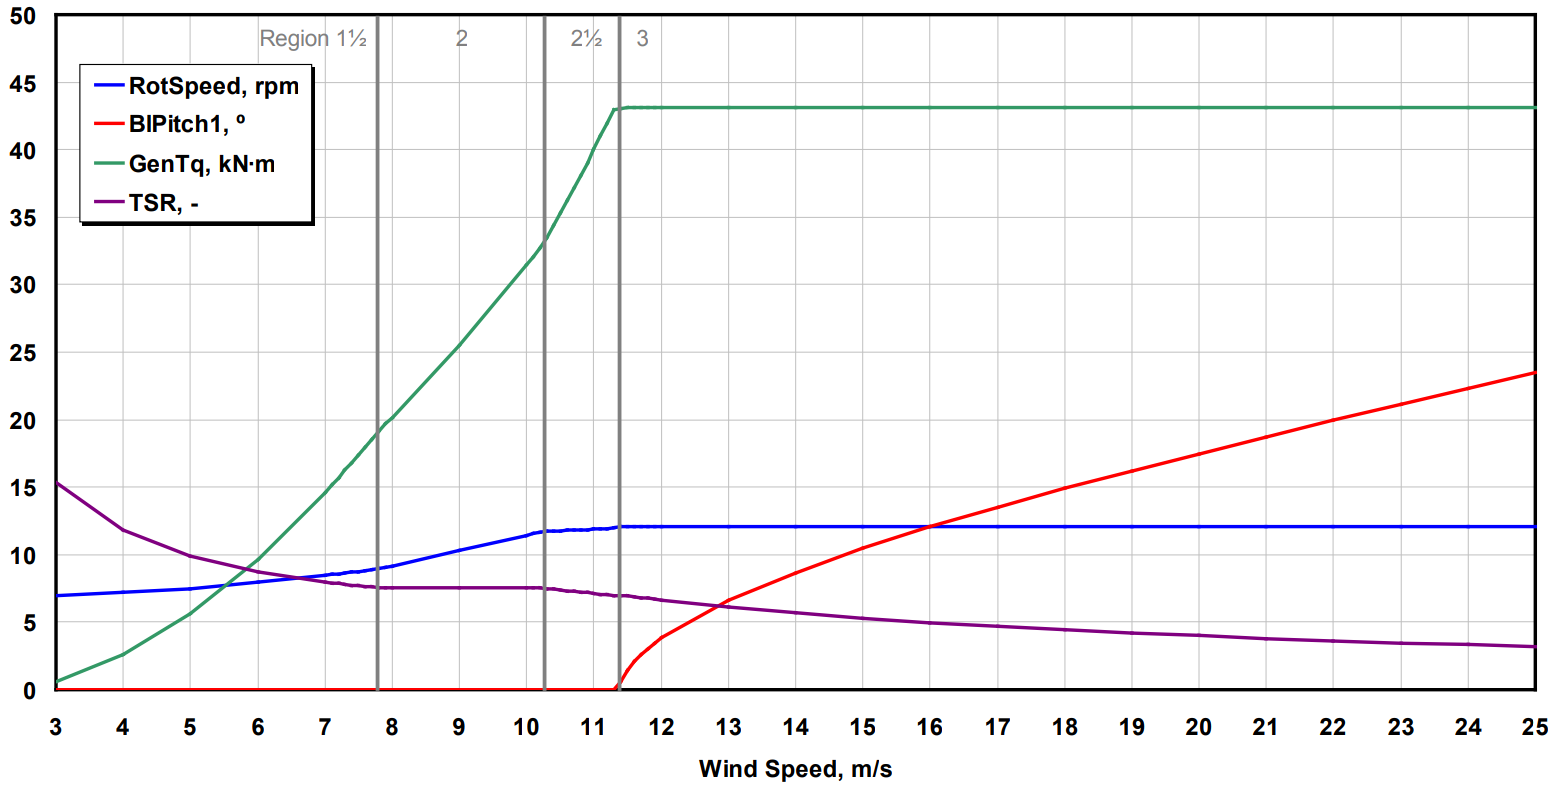
\includegraphics{NREL-5MW.png}
  \caption{Control curve of the NREL 5MW turbine, from \cite{jonkmanDefinition5MWReference2009}}
  \label{fig:nrel5mw}
\end{figure}

As described in \cite[sec 8.3]{burtonWindEnergyHandbook2011}, the normal controller design for windturbines divides the operation of a turbine into two parts, below rated and above rated. To explain this, we added reference plot of the windturbine model which we will use in our further testing, the NREL 5MW reference turbine \cite{jonkmanDefinition5MWReference2009}. Figure \ref{fig:nrel5mw} describes several properties of that turbine in relation to windspeed. Rated windspeed is a windspeed, in which the turbine gives maximum energy on highest aerodynamic effiency. In our example figure, this point is at 11.4m/s inflowing wind. At this point, the generator runs on its maximum torque (green graph) and the blades are pitched to the optimum angle of 0 degrees (red graph). At this point, the tip-speed-ratio (purple graph) is at its designed spot. When designing the turbine blades, this tip speed ratio plays an important role.
Below that windspeed, the rotor generates less rotational torque than the maximum generator torque, thus the generator torque needs to be reduced to not slow the rotor down too much. Slowing the rotor down complicates the energy generation process, and though variable-speed wind turbines allow for some play, all windturbines are limited to a certain operational range. Fixed-speed wind turbines can only run on one single rotational speed and thus need to change the torque more aggressively. In our reference turbine, you can see how the rotor speed is kept above 6.9 rpm, which is the cut-in speed of the NREL 5MW turbine. As the generated power of a windturbine is proportional to its rotor speed times generator torque, we produce less than our rated energy in this area.
Above rated windspeed, the blades need to be pitched out to stop the rotor from spinning at faster speeds than what the turbine was designed for. See the red line in the reference plot - blades are kept at zero below rated and from then on control is done only through blade pitch change. The generator torque can be kept at maximum in this area and such will also the energy production stay at maximum. To protect the turbine from damage, aerodynamic efficiency of the rotor is reduced by turning the blades along their long axis and thus moving their angle of attack against the incoming air into a less optimal range. This is done in a way that the rotational speed of the rotor stays exactly constant.

Additionally to this trivial control, optimizations to reduce vibrations and stress on the structures are implemented. The blades can be pitched individually and quickly enough to allow for different blade pitches during a single rotation of the rotor, which can be used to reduce the turbulence that hits the tower or to account for different windspeeds closer to the ground and further up in the air. Also, both generator torque and blade pitch can be used to counteract natural resonant frequencies of the structure, reducing material stress through extensive swinging of structural parts. In our 5MW reference turbine, only blade pitch is used to counteract resonances.

Usually this control is implemented by two PID controllers, which are hand-designed as described in \cite[sec 8.4]{burtonWindEnergyHandbook2011}. PID-Controllers in general have one real-valued input over time and deliver an output. This is done by calculating an error term between the input and a desired input. The output is calculated as a mixture of the error itself (P - proportional to the error), integrating the error over the last few timesteps (I - integral of the error) and calculating a derivative to the last timestep (D - derivative). The output is the sum of these 3 terms each factorized with a constant factor.
However back to windturbines. Usually, we implement two PID controllers to control a turbine, a torque and a pitch controller. Below rated windspeed, the controller for torque is active, above rated the one for pitch. The parameters to those controllers can be calculated according to the laws of control theory. Sometimes, this strong split into two operational ranges is relaxed a bit, as in the 5MW controller, the pitch part counteracts resonances also below rated speed. From this simple concept, the resulting controllers work reasonably close to theoretical maximum already. Our reference turbine has a peak power coefficient of 0.482 - meaning that at optimal wind speed, 48\% of the energy of the wind is converted into electricity. In fact, the theoretical maximum is given by the Betz limit of 59.3\% and if we account for electrical and frictional losses, the realistic maximum is even lower. So there is not much potential to be alleviated. Also, only a fraction of this potential lies in the responsibility of the control circuit. Blade design has so far been the major area for improvements.

Still, in this work, we are trying to replace these hand-designed controllers with a reinforcement-learning algorithm. We are not expecting to exceed the performance of a industry controller. So why do we even do this?

\subsection{Why we do what we do}
As you might have seen before, all controllers follow a certain style. They take a single input variable, such as rotor speed, and adjust a single output such as torque. This type of controller is called \ac{SISO}. \ac{SISO} controllers are easy to design and work reliably. They can also be interconnected, such as with the pitch controller which gets a vibration input and a rotor speed input to combine them to one output. The main challenge with wind turbine control at the moment is however not to optimize for power, but to optimize for life-time \cite[Chapter 4]{vankuikLongtermResearchChallenges2016}. The controllers are dealing well with adjusting energy to a good level, but they are missing out on keeping the windturbine intact over a long life time.

Also, the outputs get more complex. Back in the early days of wind turbines, you could control 3 variables - pitch, torque and yaw. Nowadays, we can control each of the blades individually and with a quick enough response time to wiggle the blades around within one single rotor rotation. Research on adding active control elements to the blades such as flaps is happening, which would add many more control parameters. You might have seen flaps on an aircraft wing, extending the length of the wing or adding gaps at takeoff and landing to account for the low wind speeds hitting the aircraft wing in these flight scenarios. This could also benefit wind turbines at low wind speeds. Tackling all this with \ac{SISO} is possible, but a lot of manual work.

Next, the inputs also get more complex. It is getting cheaper to install high-precision sensors, and many of them. Wind measurement techniques such as LIDAR based aenometers are able to efficiently and precisely predict incoming wind situations. Load measurements can be done in real-time across a turbine blade and in theory, it would be possible to incorporate these into control systems. However, accomodating all these input parameters in \ac{SISO} systems is difficult as we would have to hand-model each of the inputs and how exactly it ends up in the output.

We hope to lay a foundational step in solving these issues by using an end-to-end machine learning algorithm which is capable of learning a wind turbine control scenario with many inputs and outputs. Also, we must admit that we are generally interested in playing around with reinforcement learning, it's fucking cool.

\section{QBlade}
% Quickly introduce qblade as a simulation tool
Our data source in this work is the open-source simulation tool QBlade \cite{martenQBLADEOPENSOURCE2013} developed at TU Berlin. QBlade is an accessible and performant tool with the primary purpose of designing and simulating wind turbines in a graphical user interface. Its simulation results are on par with current state-of-the-art proprietary simulation tools and it yields good computational efficiency. It uses an algorithm which approximates the 3D blade structures with 2D structures and corrects the results through several error terms. Though a full CFD simulation would yield higher accuracy, our computational resources don't allow for that. To be used in reinforcement learning, we designed an interface, over which the QBlade simulation can be embedded into an external environment. Most machine-learning frameworks are written in python, so we decided to compile QBlade into library format and expose the most fundamental functions to allow it to communicate with any programming language that can load libraries. As python has a ctypes interface to load c-code, we could link a python agent to the QBlade C++ environment.

QBlade allows different simulation scenarios, for our testing we decided to only use the NREL 5MW \cite{jonkmanDefinition5MWReference2009} turbine with the default structural model and using all implemented correction mechanisms to achieve the most realistic data possible. As reference data to this turbine is easily available and publicly published by NREL, this allows us for good cross-validation.

The interface is made of 7 functions, which allow for loading a project, resetting the simulation, setting controller inputs and getting environment measurements and advancing the simulation a timestep. The observations returned in getControlVars match those that are visible to standart industry controllers, which in turn are modelled after what can be measured on a real windturbine. Concretely, we measure:
\begin{verbatim}
* rotational speed [rad/s]
* power [kW]
* wind velocity [m/s]
* yaw angle [deg]
* pitch blade 1 [deg]
* pitch blade 2 [deg]
* pitch blade 3 [deg]
* tower top bending local x [Nm]
* tower top bending local y [Nm]
* tower top bending local z [Nm]
* out-of-plane bending blade 1 [Nm]
* out-of-plane bending blade 2 [Nm]
* out-of-plane bending blade 3 [Nm]
* in-plane bending blade 1 [Nm]
* in-plane bending blade 2 [Nm]
* in-plane bending blade 3 [Nm]
* out-of-plane tip deflection blade 1 [m]
* out-of-plane tip deflection blade 2 [m]
* out-of-plane tip deflection blade 3 [m]
* in-plane tip deflection blade 1 [m]
* in-plane tip deflection blade 2 [m]
* in-plane tip deflection blade 3 [m]
* current time [s]
\end{verbatim}

Because it has no semantic meaning, we mask away current time from our reinforcement learning agent. The inputs we can give to the turbine are:
\begin{verbatim}
* generator torque [Nm]
* yaw angle [deg]
* pitch blade 1 [deg]
* pitch blade 2 [deg]
* pitch blade 3 [deg]
\end{verbatim}

After a while of experimenting with the unrestricted simulation, we added some bounds to our control parameters. Restrictions to our final version are described in section \ref{sec:alg_qblade}.

\section{Reinforcement learning}

So, why are we using reinforcement learning? We have posed the challenge earlier, that we want to learn a control system with a high number of inputs and outputs. Reinforcement learning has proven to be able to tackle high-complexity problems, both in input and output dimension. There have been successes in learning to play atari games based on pixel inputs \cite{mnihPlayingAtariDeep2013} and outperform humans, there have been successes in playing games with very long-term strategies such as go \cite{silverMasteringGameGo2016}, and research is continuing to improve. Because of all these successes, we try to automatically learn a windturbine controller.

Unfortunately, reinforcement learning isn't possible without a good amount of maths, so the following sections will be mainly mathematical.

\subsection{Environment assumptions}

At first, we need to do some assumptions on our environment $\varepsilon$. The concept environment encapsulates the reality or simulation that the reinforcement learning algorithm works in. This could be an actual cyber-physical system or a simulation. The first assumption to this environment is that this system operates over time and we can discretize time into timesteps. Our environment here is the simulated wind turbine, but it could be a computer game \cite{lillicrapCONTINUOUSCONTROLDEEP2015}, a physics simulation\cite{brockmanOpenAIGym2016} or even an actual existing wind turbine \cite{kolterDesignAnalysisLearning2012}. 
In every timestep, the environment supplies us with an observation \(x\) and a scalar reward \(r\) for taking an action \(a\) in that state. In theory, the full trajectory \((x_0, a_0, ..., x_t)\) could be needed to describe the full state of the simulation at timestep t \(s_t\). However, the algorithms we looked at assume that the state progressions can be modelled as a \ac{MDP} of observations, as in that what will happen at timestep t+1 is only dependent on the observation at timestep t, not also on for example t-10. In \ac{MDP}, the state transition probability \(p(x_{t+1}|x_t, a_t)\) is fully descriptive, as in it is equal to \(p(x_{t+1}|x_0, a_0, ..., x_t, a_t\). Because we assume the observation \(x\) to be fully descriptive, we will use the term state as equivalent to observation \(s_t = x_t\). In reality, the observed state doesn't have to represent the entirety of the state of the simulation, in fact it usually is only a small subset. For our wind turbine example, the observed state is limited to what can be measured with sensors on a wind turbine, in an arcade game it could be the pixel output or in a physical simulation it could be some key values in the simulation. We denote the probability of a state transition to a specific $s'$ as $p(s'|s,a;\varepsilon)$ and the distribution over all states $s'$ as $P_{s' \sim \varepsilon | s,a}$ and when $s,a$ is clear, we omit it.

The reward \(r(s,a)\) is a scalar value which judges the action $a$ taken in the current state $s$ of the simulation. A higher reward means the action is better than that of a lower reward. Sometimes, the reward function is obvious from the system, as in an arcade game it would surely be the score or in chess it could be 1 for win, -1 for lose and 0 for not decided yet. In both cases, sometimes a certain timespan passes before a reward for an action kicks in, which is also to be learned. In our paper, we will dedicate a section on how we designed our reward function, whereas in general reinforcement learning theory, it is assumed to exist and be supplied by the environment.

Additionally to the state and reward, an environment can optionally send out a done signal \(d\), which indicates a state in which further simulation is not possible and the environment wants to be reset to an initial state. In a chess game, this would be a loss or a win, and with a windturbine that could for example be fatal structural damage. 

In every timestep, the agent supplies an action \(a\). This action could be button presses in an arcade game or blade pitch in a windturbine simulation. The mission of the agent is to pick actions which maximize cumulative reward. In other words, it should steer the environment to achieve best performance. Let's write down this mission. We want to maximize:

\begin{equation}
J = \mathbb{E}r
\end{equation}

This formula is still a bit incomplete - we didn't yet specify our expectation. And wasn't reward defined on states and actions? But that is because we are still missing some definitions. Luckily, there are some ahead.

\subsection{Definitions}
\label{sec:definitions}

Additionally to the terms defined by the environment, we introduce some terms which are common to reinforcement learning
\begin{itemize}
  \item \textbf{Policy} A function that maps from states to actions. There are deterministic policies $\mu: S -> A$ and stochastic policies $\pi: S -> P(A)$. If we approximate a policy by a function approximator parametrized with $\theta$, we write $\pi(s;\theta)$ or omit the parameters when clear.
  \item \textbf{Value} A value with respect to a policy and a starting state s gives the accumulative reward of following that policy from state s until infinitely in the future. $V^{\pi}(s_t) = \mathbb{E}_{s_i \sim \varepsilon, a_i \sim \pi, i>t} r(s_i, a_i) $. As we have a stochastic environment and policy, we have to add an expectation term over actions taken and states resulting from those actions. It is the expected accumulative reward of following that policy. Furthermore a value can be discounted or undiscounted. Discounting means we multiply a discounting factor $\gamma \in [0,1]$ to rewards in the fashion of $r_0 \gamma^0 + r_1 \gamma^1 + r_2 \gamma^2 ...$, which results in distant future rewards being weighted less than closer ones.
  \item \textbf{Return} If we measured a value function, that would be the return. Obviously we can't measure infinitely, so a return is only defined on a finite trajectory of state-transitions, but otherwise is equal to a value.
  \item \textbf{Optimal policy} The theoretical construct of a policy that always takes the best action with respect to accumulative reward. Though we rarely know this policy, there must always be at least one policy which gives the highest value of all possible policies in a finite \ac{MDP}
  \item \textbf{Q-Value} The reward of taking action a in state s plus the value following a policy after that $Q^{\pi}(s,a) = r(s, a) + \mathbb{E}_{s' \sim \varepsilon} V^{\pi}(s')$. When following the optimal policy, we simply write $Q^*(s,a)$. Usually, our Q functions are discounted. Note that we can also define Values on Q-Values: $V^{\pi}(s) = \mathbb{E}_{a \sim \pi} Q(s, a)$. If we approximate Q by a function approximator parametrized with $\theta$, we write $Q(s, a;\theta)$ or omit it in case it is clear.
  \item \textbf{Actor-Critic} Actor is just another name for a learnt policy and critic just another name for an estimated Q-Value function. These two frequently appear together, if that happens we are using an actor-critic algorithm.
  \item \textbf{State-density} According to \cite{suttonPolicyGradientMethods}, $d^{\pi}(s) = \lim_{t -> \infty} p(s_t = s | s_0, \pi)$ describes how likely it is to be in state s when following a policy $\pi$ forever. If we for example have a policy which plays go as well as the authors of this paper, states with a lot of enemy stones and very few own stones might be very likely, and a state without enemy stones at all would be very unlikely. Also according to \cite{suttonPolicyGradientMethods} this distribution is independent of the starting state $s_0$ and only dependent on the policy and of course the environment. In later papers, commonly a discounted version of this is used. $\rho^{\pi}(s)$ weights future probabilities less and thus can be described as the probability of being in state s \textit{soon} when following policy $\pi$. We will omit a precise definition here, you can look it up at \cite[Section 2.1]{silverDeterministicPolicyGradient2013}.
\end{itemize}

Now, with all these definitions at hand, we can specify our mission a bit better. We want to maximize
\begin{equation}
J^{\pi} = \mathbb{E}_{s \sim \rho^{\pi}, a \sim \pi}r(s, a) = \int_S \rho^{\pi}(s) \int_A \pi(s) r(s, a)
\label{equ:maximize_rewards}
\end{equation}

In other words, we want a very high probability of being in a state ($\rho^{\pi}$) which might give good rewards, and in that state we want a high probability of taking an action ($\pi$) which might give a good reward. In our wind turbine, rewards could for example be the all the costs and incomes summed together, so at every point in time we could count income by energy yield or costs because of maintenance (with our controller more likely costs for rebuilding the entire turbine). This work would be easy if we could directly calculate this equation but clearly, there is a bit of a problem ahead. Firstly, we don't know $\rho$ as we don't exactly know the environment we are modelling. We can observe some rewards, states and actions, but only very few of them. We might then see that using 0.3MN of torque at rotational speed 11rpm yields good energy yield, but how about rotational speed 11.1rpm? We might have never seen that. Also, rotating the turbine at 15rpm might be a good strategy to immediately achieve high power outputs, but we might need to fix our turbine after running this policy for just a few days and incur a heavy penalty. So we don't know how rewards will spread out in the future. Luckily we have defined Q-Values above. We could use them somehow, so let's discuss how to learn them.

\subsection{Q-Learning}

At first we will present a very basic algorithm for a Q learning agent, which is based on the basic Bellman-Equation \cite{bellmanTheoryDynamicProgramming1954}. It is proven, that

\begin{equation}
Q^*(s, a) = \mathbb{E}_{s' \sim \varepsilon | s,a}[r(s,a) + \gamma\max_{a'}Q^*(s', a')]
\end{equation}

converges to the optimal solution when using iterative value updates. We will quickly explain this Bellman Equation. This equation uses the notion of a state-value function, also called Q function. In the Bellman Equation, it describes the total accumulated return until infinity taking an action $a$ in state $s$, receiving reward $r$, ending up in state $s'$ and then following the optimal policy afterwards. $\gamma$ acts as a discounting factor just as in our return function. It is even possible to implement an algorithm from this. We could create a lookup table for all s and a, initialize it all zero and whenever observing a state transition, we could update the table at that state and action after the above notation.

With the help of this function, we can compare different actions in our current state. However, this table is only computationally feasible when we have small finite state and action spaces. If any of the two spaces is big or even continuous, we have to replace the table by an estimator for Q.

Even with an estimated Q, though no longer guaranteed, we can still converge towards the optimal solution. For training an estimator, we need a loss which we can derive. For this, we define our learning target for learning step i as
\begin{equation}
y_i = \mathbb{E}_{s' \sim \varepsilon}[r + \gamma \max_{a'}Q^*(s', a';\theta_{i})]
\end{equation}
For the moment, let's assume we can still calculate $\max_{a'}$. In fact, in a small finite action space we could just try all possible values of a. Our $y$ is then the current reward added to the highest possible rewards in the future, with other words exactly what we want to have as Q. We use the parameters $\theta_{i}$ in the target, so in theory, when deriving a later loss, we would also have to derive over our targets. However, in Q learning, this is commonly ignored.

Now, on our learning target y, we can define a loss as
\begin{equation}
L(\theta_i) = \mathbb{E}_{s \sim \varepsilon}[(y_i - Q^*(s, a;\theta_i))^2]
\end{equation}
This already looks close to some squared error term. To calculate the expectation value over the environment $\varepsilon$, we need to do some form of Monte-Carlo experiment, in which we approximate that expectation value by repeatedly drawing samples from the underlying distribution. Luckily, we can easily draw samples from our environment, and we can even reuse old samples. Thus we store all samples in a replay buffer and uniformly draw from it to resemble a Monte-Carlo experiment. 

Deriving for $\theta_i$ and applying the chain rule, we get the loss derivative
\begin{equation}
\Delta_{\theta_i} L(\theta_i) = \mathbb{E}[(y_i - Q^*(s, a;\theta_i))\Delta_{\theta_i}Q^*(s, a;\theta_i)]
\end{equation}
Using our Monte-Carlo like batch from the replay buffer, we end up with stochastic gradient descent.

Thus we just derived a method to train a Q function under the assumption of an optimal policy. In \cite{mnihPlayingAtariDeep2013}, the authors assumed a finite state space and could use the greedy policy $argmax_a Q(s', a)$ by searching the entire action space. We are presented with an infinite action space though, which is why we can't implement a greedy policy without high computational expense. So, for our work, we have to also learn a policy and not just a Q estimator. So let's try to derive a way to learn a policy.


\subsection{Policy Gradients}

We will at first give an intuitive explanation of a basic algorithm which forms the basis for many modern reinforcement learning algorithms, including the one we chose. The algorithm is called \ac{REINFORCE} (no joke) and was originally presented by \cite{williamsSimpleStatisticalGradientfollowing}. Then we will add a Q term to it according to \cite{suttonPolicyGradientMethods} and call it \ac{PG}. \cite{degrisOffPolicyActorCritic2013} generalized that term and made an off-policy version of policy gradients, which we will not discuss in detail. That version was then used by \cite{silverDeterministicPolicyGradient2013} and the stochastic policy was replaced by a deterministic one, the algorithm was called \ac{DPG}. This algorithm finally lays the basis for \ac{DDPG} by \cite{lillicrapCONTINUOUSCONTROLDEEP2015}, which is what we used to start our experimentation.

Let's assume we have a probablistic policy $\pi: S \rightarrow P(A)$ which is parametrized by $\theta$. An intuitive way of improving this policy could be to increase the gradient proportional to the reward an action yielded:
\begin{equation}
\theta_{i+1} = \theta_i + \alpha r(s,a) \Delta \pi_{\theta_i}(a|s)
\label{equ:reinforce}
\end{equation}
We could do this for all states we see and would end up with an iterative way of improving our policy. In fact, this is similar to the \ac{REINFORCE} algorithm (if we add our importance sampling trick from below). However, we might not know rewards for any action, state or have noisy rewards. Luckily, we derived Q-Learning in the section before and thus have an estimation which action will give which return in this step. So, with our newly gained Q, for all actions and states, do
\begin{equation}
\theta_{i+1} = \theta_i + \alpha Q(s, a)\Delta \pi_{\theta_i}(a|s)
\end{equation}
This way, actions with higher Q values will receive a higher gradient step. As Q is constant with respect to $\theta$ we don't have to derive along Q here. Problematic is though, that the Q term we used, always took the best possible actions, which could be vastly different from the actions under our policy. Thus, we need to reformulate Q to account for our policy instead of the optimal policy

\begin{equation}
Q^{\pi}(s, a) = \mathbb{E}_{s' \sim \varepsilon, a' \sim \pi | s,a}[r + \gamma Q^{\pi}(s', a')]
\end{equation}

Now, in theory, we can not regard Q as constant with respect to $\theta$ anymore, because it is dependent on the policy. \cite{suttonPolicyGradientMethods} claim though that it can be ommitted and still regarded as constant. However there is still a problem if we integrate this new Q into our policy updates. We assume that we use the same $\pi$ for exploration while doing training, so this policy is responsible for taking actions in the environment and also responsible for which experiences we see during our training. So let's assume the policy is poorly initialized at the beginning of our training and gives action 1 a probability 4 times as high as action 2, though taking action 2 would yield a 10\% better return in our Q function. Now, as we are taking action 1 4 times as often as action 2, we will also perform gradient updates on action 1 4 times as often in our Monte-Carlo expectation draw. Though each of the gradient update steps is smaller due to the lower Q factor, the higher frequency of updating action 1 will lead to action 1 getting an advantage over action 2 in this update strategy. To correct for this oversampling bias, we could employ a trick which is called importance sampling. Because we know the bias from the probability distribution of our policy, we divide that probability from the update term:
\begin{equation}
\theta_{i+1} = \theta_i + \alpha Q^{\pi}(s, a) \frac{ \Delta \pi_{\theta_i}(a|s)}{\pi_{\theta_i}(a|s)}
\end{equation}
We might remember from calculus that $\frac{\Delta x}{x} = \Delta \log x$ so we simplify to
\begin{equation}
\theta_{i+1} = \theta_i + \alpha Q^{\pi}(s, a) \Delta \log \pi_{\theta_i}(a|s)
\label{equ:pg_update}
\end{equation}

So, let's sum up what we have done before and formulate our goal again. Before, we ignored for brevity that we are dealing with expectation calculations and that we are doing these updates under a stochastic environment, so to write it down formally correct, we need to remember the density function of a state under a policy from section \ref{sec:definitions}. Using the discounted version approximates the Monte-Carlo experiments we are doing better than the undiscounted version, as effectively we do not train forever on one constant policy, but change it frequently, so we will use $\rho^{\pi}$ to approximate how likely we are in a state $s$ when using policy $\pi$.

Having this $\rho$, let's write our objective function $J$ which we want to maximize.
\begin{equation}
J(\pi) = \int_S \rho^{\pi}(s) \int_A \pi(s, a)Q^{\pi}(s, a) dads = \mathbb{E}_{s \sim \rho^{\pi}, a \sim \pi}[Q^{\pi}(s,a)]
\end{equation}
This looks similar to equation \ref{equ:maximize_rewards}, just that we use Q now.


\cite{suttonPolicyGradientMethods} proves that deriving this yields
\begin{equation}
\Delta J(\pi) = \mathbb{E}_{s \sim \rho^{\pi}, a \sim \pi}[\Delta \log \pi(a|s)Q^{\pi}(s, a)]
\label{equ:pg}
\end{equation}
This equation is very famous in reinforcement learning and is called policy gradients. And by coincidence, it is equivalent to what we intuitively derived in equation \ref{equ:pg_update}. We decided to skip the actual proof and use this intuitive explanation instead, and we used the intuitive explanation in \cite[Chapter 13, Section 3, after Equation 13.8]{suttonReinforcementLearningIntroduction2018} to explain the nature of this policy gradient equation.


In reinforcement-learning, it has proven helpful to do off-policy learning, in which another policy $\beta$ than the one being trained can generate experiences. We would then reformulate our expectation to $\mathbb{E}_{s \sim \rho^{\beta}, a \sim \beta}$. Thus, we could store past experiences in a replay buffer and learn from that. In fact, we were already able to use a replay buffer in the Q learning part. If we wanted to do that on our policy however, we would need to correct for the bias of the other policy aswell with importance sampling. However we will not derive stochastic off-policy updates, because using the \ac{DPG} algorithm, this problem is solved. If you want to learn about \ac{Off-PAC} with stochastic policies, we recommend to read \cite{degrisOffPolicyActorCritic2013}

Additionally to this problem, another problem will be solved by \ac{DPG} as well: If we remember our Q expectation term, in which actions were sampled from the policy $\mathbb{E}_{a \sim \pi}$. We needed this expectation term, because we were dealing with stochastic policies. If instead learning deterministic policies, we can exclude policy expectation from the equation. But before going through all the advantages of deterministic policies, let's first explain it.

\subsection{Deterministic Policy Gradients}

Before \cite{silverDeterministicPolicyGradient2013}, stochastic policies were preferred because the stochastic nature aided exploration and because there was simply no theory on how to derive deterministic policy gradients. The idea behind deterministic policy gradients is to replace the stochastic policy $\pi: S -> P(A)$ with a deterministic one $\mu: S -> A$. Also, we are switching from small finite action spaces to continous action spaces. Now, updating this policy according to the equations above does not work anymore due to two problems. At first and most significantly, above we needed all $a$ or at least some form of maximization to calculate the full gradient of $\pi(a|s)$. This is difficult with a continous action space now. Furthermore our importance sampling trick, our correction for overestimation bias based on the bias of the policy, does not work anymore. We don't now the bias of that policy, because it is deterministic and will yield only a single action for any state. 

So, following the policy gradient has become difficult. However, let's have a look at our Q function. We can replace our stochastic policy with a deterministic one and get

\begin{equation}
Q^{\mu}(s,a) = \mathbb{E}_{s' \sim \varepsilon | s,a}[r + \gamma Q^{\mu}(s', \mu(s'))]
\end{equation}

Now, our Q is only calculating an expectation on the environment distribution, not anymore both on $s' \sim \varepsilon, a' \sim \pi$. This is an advantage, because computing only one expectation requires less samples and we do not have to worry for any bias from the policy in Q-updates. When we do our Monte-Carlo experiments to update it, we can take our generated samples from the environment and assume they are modelling the underlying environment.

If we are visualizing our Q as a function of state and action, we get a fully differentiable surface. If we derive this surface along the action dimension, we get a gradient which points in the direction of a better action for this state. We could direcly follow this gradient and calculate our policy update from it:

\begin{equation}
\theta_{i+1} = \theta_i + \alpha \mathbb{E}_{s \sim \rho^{\mu_{\theta_i}}}[\Delta Q^{\mu_{\theta_i}}(s, \mu_{\theta_i}(s))]
\end{equation}

\cite[Theorem 1]{silverDeterministicPolicyGradient2013} proves that this gradient always exists. We now managed to remove any expectation that is related to our action space from our gradient updates. This is beautiful because at first, we do not have to sample over many actions to learn this expectation. But more importantly, this term also works off policy, and without importance sampling. We can use a different exploration policy $\beta$ and replace our expectation term $\mathbb{E}_{s \sim \rho^{\mu}}$ with $\mathbb{E}_{\rho^{\beta}}$ here completely unpenalized. Why is this so? \cite{degrisOffPolicyActorCritic2013} proved off-policy gradients possible, but had to use importance sampling to correct for the bias in $\beta$. In fact, generally, it is not possible to do this replacement. However, \cite[Section 4.3]{silverDeterministicPolicyGradient2013} formulated a compatibility theorem. They proved, that a linear function approximator $Q^{\omega}$ which minimizes the MSE between $Q^{\omega}$ and $Q^{\mu}$ will retain the gradient, even when trained on samples generated by $\beta$, and called this Q \textit{compatible}. However, in practice we are not minimizing that loss and neither are we using linear function approximators. \cite{bhatnagarConvergentTemporalDifferenceLearning2009} proved that using a non-linear function approximator to predict the value function $V(s)$ will converge towards a local optimum. As we can formulate our Q by using V, we transfer this to our scenario. However, \ac{DPG} is not definitely proven to converge for a non-linear function approximator, as this transfer was, to our knowledge, never fully formulated. Observations show that it still does converge.

So let's restate our objective function for the actor.

\begin{equation}
J(\mu_{\theta}) = \int_S \rho^{\beta}(s) Q^{\omega}(s,\mu_{\theta}(s)) ds = \mathbb{E}_{s \sim \rho^{\beta}}[Q^{\omega}(s,\mu_{\theta}(s))]
\end{equation}


\subsection{DDPG}

\begin{figure}
  \centering
  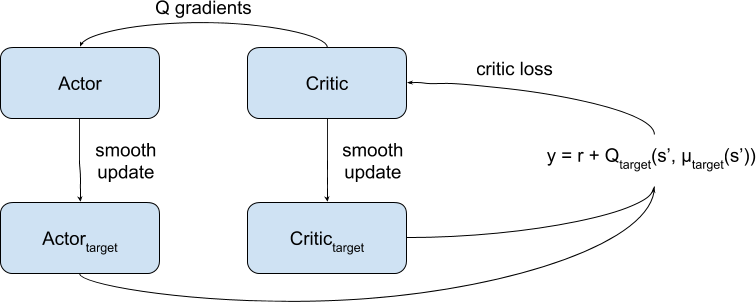
\includegraphics[width=0.6\linewidth]{DDPG_Setup.png}
  \caption{DDPG Network}
  \label{fig:ddpgsetup}
\end{figure}

\ac{DDPG} is a combination of \ac{DPG} and \ac{DQN}. \cite{lillicrapCONTINUOUSCONTROLDEEP2015} tackle several problems in the two algorithms to combine them. At first, traditional Q learning updates the Q network parameters based on a target $y$ calculated on the Q network parameters themselves. This introduces instability and to tackle this, \cite{mnihPlayingAtariDeep2013} introduced a second Q network $Q'$ which they call target network, for which the parameters are held constant over a period of updates. They calculate the $y$ based on the second network $Q'$. After a number of steps, the parameters from the actual Q network are then copied over to the target. The stability gain in their paper depends greatly on the number of steps after which to perform an update. In \ac{DDPG}, they instead use smooth target updates, where every step, the parameters of the actual network fade over to the target: $\theta_{target} = \tau \theta + (1 - \tau) \theta_{target}$. The fade-over parameter $\tau$ was recommended to be set to a small number like 0.001. Additionally to the target Q-network, they also found that a target policy $\mu'$ improves stability, and they update it the same way as the main policy. But this is a lot at once. Let's have a look at the Q update functions

\begin{equation}
y = r(s, a) + \gamma Q'(s', \mu'(s';\theta^{\mu'});\theta^{Q'})
\end{equation}
\begin{equation}
L(\theta^Q) = \mathbb{E}_{s \sim \rho^{\beta}, a \sim \beta, s' \sim \varepsilon}[(Q(s, a;\theta^Q) - y)^2]
\end{equation}


We sketched an overview in figure \ref{fig:ddpgsetup}. Remember that actor was another name for policy and critic another name for Q estimator. Notice how for calculating the Q targets, they used both the target actor $\mu'$ for generating actions which are then evaluated by the target critic $Q'$. This is their version of the improvement over \ac{DQN} for their instable Q function, as they also observed instabilities. Note how the Q function here does not really predict the value of following a specific policy anymore, as before we could always denote which policy Q was trained on. Also, this Q is approximated by a non-linear function approximator instead of the linear one from compatible \ac{DPG}. \cite{lillicrapCONTINUOUSCONTROLDEEP2015} do not provide a proof of convergence for this new, mixed Q update. Still, we have an off-policy way of improving the critic now. The actor is directly copied from \ac{DPG} even though it does not fulfil the \textit{compatible} property.

\begin{equation}
J(\theta^{\mu}) = \mathbb{E}_{s \sim \rho^{\beta}}[Q(s, \mu(s;\theta^{\mu});\theta^Q)]
\end{equation}

Let's derive these two equations. First the policy gradient:

\begin{equation}
\Delta_{\theta^{\mu}}J(\theta^{\mu}) = \mathbb{E}_{s \sim \rho^{\beta}}[\Delta_{\theta^{\mu}}Q(s, \mu(s;\theta^{\mu});\theta^Q)] = \mathbb{E}_{s \sim \rho^{\beta}}[\Delta_a Q(s, a;\theta^Q | a=\mu(s)) \Delta_{\theta^{\mu}}\mu(s;\theta^{\mu})]
\end{equation}

And the Q update:
\begin{equation}
\Delta_{\theta^Q} L(\theta^Q) = \mathbb{E}_{s \sim \rho^{\beta}, a \sim \beta, s' \sim \varepsilon}[(Q(s, a;\theta^Q) - y)\Delta_{\theta^Q}Q(s, a;\theta^Q)]
\end{equation}

Similar to other reinforcement learning algorithms, we will again not compute the full gradient but use stochastic gradient ascend with batch learning. To rephrase gradient ascend to gradient descend, they multiply the policy loss with $-1$. In fact, in the original \ac{DDPG} algorithm, they used Adam \cite{kingmaAdamMethodStochastic2017} optimization instead of stochastic gradient descend. As activations, they used relu \cite{agarapDeepLearningUsing2019}. Their network architecture for the actor consisted of two fully connected layers with 400 and 300 units and instead of relu they used tanh activations in the last layer to bound actions. For the critic, they had a version which learnt upon pixel outputs and used convolutional layers, while we only look at the low-dimensional version. For this, they also used a two layer variant with 400 and 300 units. State inputs were fed through the whole network, while actions were concatenated in onto the second layer, skipping the first.

Furthermore, to aid exploration, they added noise in form of a Ornstein-Uhlenbeck process \cite{uhlenbeckTheoryBrownianMotion1930}.

For readability, we added a copy of their algorithm in Algorithm \ref{alg:vanilladdpg}, with minor adjustments to fit our notation.

\begin{algorithm}
\SetAlgoLined
Randomly initialize critic network $Q(s, a;\theta^Q)$ and actor $\mu(s;\theta^{\mu})$ with weights $\theta^Q$ and $\theta^{\mu}$\\
Initialize target networks $Q'$ and $\mu'$ with weights $\theta^{Q'} \leftarrow \theta^Q, \theta^{\mu'} \leftarrow \theta^{\mu}$\\
Initialize replay buffer $\mathcal{R}$\\

\For{episode = 1, M}{
  Initialize a random process $\mathcal{N}$ for action exploration\\
  Receive initial observation state $s_1$\\
  \For{t = 1, T}{
    Select action $a_t = \mu(s_t;\theta^{\mu}) + \mathcal{N}_t$ according to the current policy and exploration noise\\
    Execute action $a_t$ and observe reward $r_t$ and observe new state $s_{t+1}$\\
    Store transition $(s_t, a_t, r_t, s_{t+1})$ in $\mathcal{R}$\\
    Sample a random minibatch of $N$ transitions $(s_i, a_i, r_i, s_{i+1})$ from $\mathcal{R}$\\
    Set $y_i = r_i + \gamma Q'(s_{i+1}, \mu'(s_{i+1};\theta^{\mu'});\theta^{Q'})$\\
    Update critic by minimizing the loss: $L = \frac{1}{N} \sum_i (y_i - Q(s_i, a_i;\theta^Q))^2$\\
    Update the actor policy using the sampled policy gradient: $\Delta_{\theta^{\mu}} J \approx \frac{1}{N} \sum_{i} \Delta_a Q(s_i, a;\theta^Q | a=\mu(s_i)) \Delta_{\theta^{\mu}}\mu(s_i;\theta^{\mu})$\\
    Update the target networks:\\
    $\theta^{Q'} \leftarrow \tau \theta^{Q} + (1-\tau)\theta^{Q'}$\\
    $\theta^{\mu'} \leftarrow \tau \theta^{\mu} + (1-\tau)\theta^{\mu'}$
  }
}
\caption{Vanilla DDPG algorithm}
\label{alg:vanilladdpg}
\end{algorithm}

\section{RL on windturbines}
We are aware of one paper \cite{kolterDesignAnalysisLearning2012} which tried RL on windturbines already, we want to dedicate a section to it. The team behind that paper built a miniature model of a windturbine and used a variation of the \ac{REINFORCE} algorithm to control it.

\begin{figure}
  \centering
  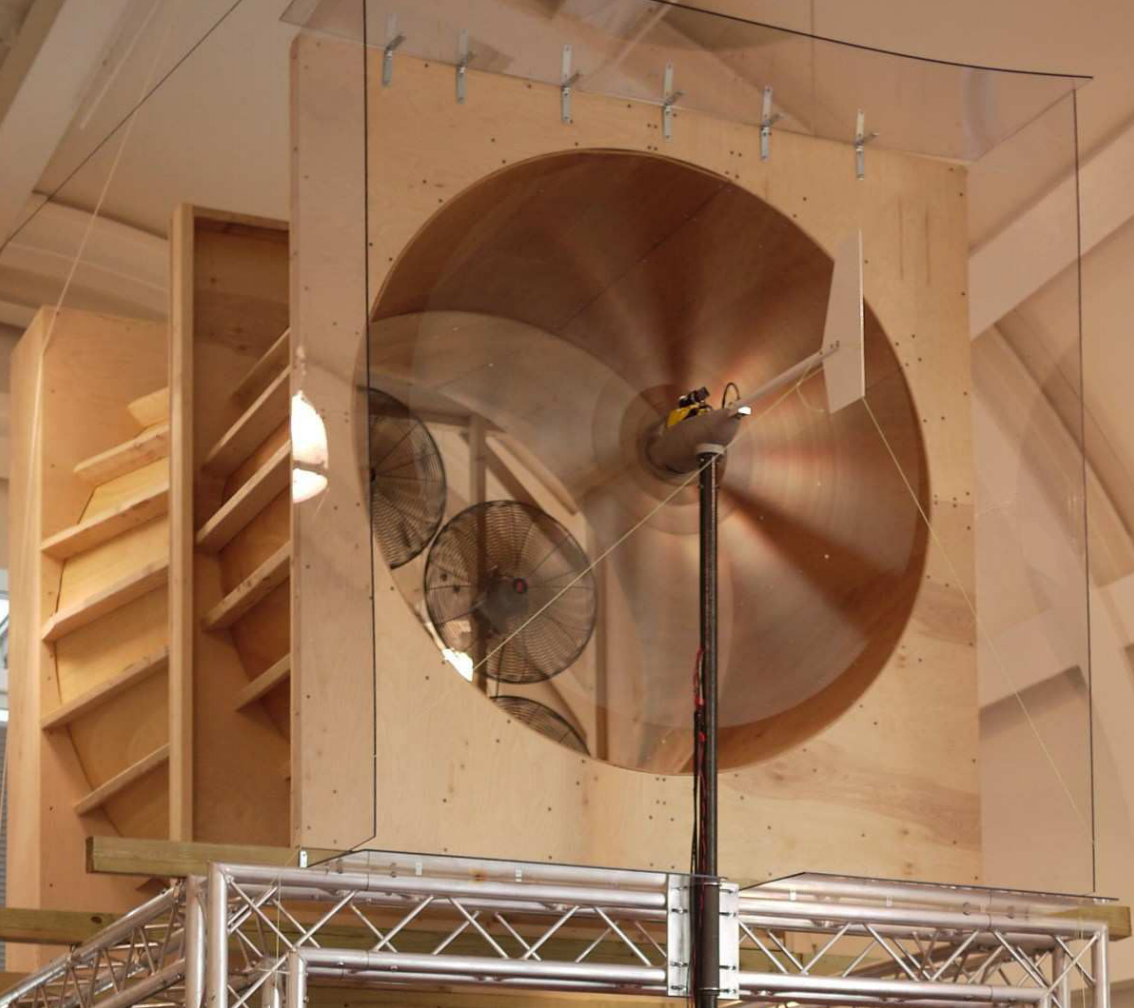
\includegraphics[width=0.5\linewidth]{Miniturbine.png}
  \caption{The mini wind-turbine from \cite{kolterDesignAnalysisLearning2012}}
  \label{fig:miniturbine}
\end{figure}

Their miniature model was built from cheap and low-scale parts, they simulated a wind-tunnel by attaching several fans in front of a wooden tube and at the end placed their turbine. Figure \ref{fig:miniturbine} illustrates this. Each of the blades of that miniature turbine is individually controllable and through a correction term, they are able to achieve independent pitch control which is able to pitch the motors to a value based on rotor position. Though this turbine rotates many times faster than a normal, full scale wind turbine, the underlying principles are the same (500rpm vs 11rpm). For us most importantly, they used reinforcement learning to control this turbine.

As training input, they used a single observation in contrast to popular reinforcment learning which operates on high-dimensional observation space. This observation was power output of the turbine, and they treated it as reward to the system, not having any state observations. Their action space consisted of electrical load on the generator and blade pitch, which was uniformly applied to all 3 blades. In fact, they designed their policy as to return a gaussian distribution over these two parameters directly without any input: $\pi: \varnothing \rightarrow P(\mathbb{R}^2)$. To run the training, they kept the wind speed constant, let the turbine spool up to speed and then let it run with a set of parameters returned by the policy. They ran these parameters for 2 seconds on the turbine, averaged power output over that time into a reward and then ran an iteration of their algorithm to generate new parameters, starting with random parameters. 
They first tested the \ac{REINFORCE} algorithm, with operates without a Q network and trains a policy directly on rewards. This algorithm was discussed above and utilizes the following gradient equation:

\begin{equation}
\Delta_{\pi^{\theta}} J = \mathbb{E}_{a \sim \pi, r \sim \varepsilon | a} r \Delta \log \pi(a;\theta)
\end{equation}

Note, how they denoted J in their paper as rewards, while we are using r for rewards and J for objective functions. Also, they used $\omega$ as a symbol for the action taken, while we use $a$. Also note how their policy is not dependent on a state but directly predicts actions. They did not explicitely note what they formulated their expectation term on, but we added it here for clarity. Note the similarity to what we discussed in equation \ref{equ:reinforce} and \ref{equ:pg}. In addition to this, they came up with an algorithm which they call Trust Region Policy Search, and which is astonishingly different from Trust Region Policy Optimization. With a few additions, they incorporated off-policy learning and second order error approximation into their algorithm, and showed later that it performs nicely. They were able to find optimal pitch and load settings as soon as 15 timesteps after the start of the simulation.

Having described this paper, we want to also summarize what we do differently and why. First, they had a simpler environment. While a full scale windturbine has a strong tendency to destroy itself when outside of their operational margin, their turbine did not fly apart when not applying braking. Also, they were setting electrical resistance, not rotor torque. This system applies a braking force constant to rotational speed times resistance parameter, and thus already acts as a P controller. We were setting torque, so we had to adjust it regularly to rotor speed. In general, their turbine behaved more concavely opposed to our turbine, which with a constant parameter set, would settle to either rotating quickly backwards, forwards or not at all. Because of this, they were able to give the turbine some time at the beginning to stabilize before applying reinforcement learning while we needed to start with the standing turbine. Lastly and most importantly, they aimed to find optimal control settings for a constant wind speed. To create a full controller setup from this, they would have to repeat this process for every windspeed and use the resulting look-up table to derive a PID-controller. We however want to create an end-to-end system and want to experiment with the possibly higher expressive nature of predicting actions based on a full state input. We want to create a version as general as possible. Also, as \ac{DDPG} is a direct successor on \ac{REINFORCE} and has proven to outperform it in many areas, we do not reimplement their paper.

\chapter{Experimentation}

For everyone who is interested in a recap of our design process, in this section we will provide such. We will again present our algorithm in a later section. To understand our design decisions, it might be interesting to read this passage, but you can also skip this passage and just read the rest. 

\section{Gym Experiments}

At the start of our experimentation, we took off with a well-known problem and a proven implementation. We used the OpenAI-Pendulum task, in which a pendulum in gravity needs to be held upright by applying a force to it. OpenAI Gyms generally serve as benchmarks for reinforcement learning algorithms and most foundational papers and articles evaluate their solutions based on how well they perform in OpenAI Gyms. We managed to find a solution with our DDPG implementation. We hoped that the implementation might yield results on our windturbine environment as well and exchanged the OpenAI gym for qblade.

The first runs looked marvellous, perfectly holding rated speed, until we found out that those perfect values were prescribed by a setting in the qblade project file, and disabling this setting marked the beginning of our actual experimentation phase.

\section{Starting with qblade}

On our first experimentation steps, we did not yet have experience with how the qblade simulation behaves with a random or not well designed controller. Our observation was, that the simulation was resting between two different states, which we want to call \ac{FMM} and \ac{BMM}.

\ac{FMM} is characterized by a rotational speed of ca 5 times rated speed, at 4.3 rad/s. At this speed, for some reason, the rotor will not speed up anymore. However, severe vibrations and sometimes the case of a disjointed blade happen. Especially in the case of a blade flying off, deflection values skyrocket up to several orders of magnitude higher than values seen in normal operation, and with one or more missing blades, the rotor will quickly stop rotating. This state is usually reached by a too low generator torque while not pitching out blades and sometimes stays stable for several thousand steps until a blade falls off.

\ac{BMM} is characterized by a negative rotational speed, up to -3.8 rad/s. This can be reached by setting a higher generator torque than the rotor torque which is produced by aerodynamic lift on the blades. Also in this state, extreme vibrations and sometimes blades flying off can be observed, and like \ac{FMM} this state is stable until a blade falls off. 

In neither of these modes, the simulation is within realistic bounds and the observations gotten from the simulation at this part are not credible. After we observed that the controller itself wasn't able to avoid these states on its own, we inhibited reaching these states by outputting a death condition when being in negative rotational areas or high positive. After a death, the simulation gets reset to initial state and the controller has more chances to learn.


\section{Designing reward functions}
\label{rewardfunctions}

As qblade doesn't provide a built-in reward function, we needed to craft our own reward function based on the observed state. We considered several possible variants. We will first introduce all of them and give a more detailed explanation later

\begin{itemize}

\item \textbf{Rated speed} Hold a rated speed. Observe current rotational speed \(s_{rot}\) and with given rated speed \(s^*_{rot}\) calculate reward \(r(s) = -\abs{\frac{s_{rot} - s^*_{rot}}{s^*_{rot}}}\)

\item \textbf{Rated power} Hold a rated power. Observe current power \(s_{pow}\) and with given rated power \(s^*_{pow}\) calculate reward \(r(s) = -\abs{\frac{s_{pow} - s^*_{pow}}{s^*_{pow}}}\)

\item \textbf{Maximal power} Generate the maximum power possible. Observe current power \(s_{pow}\) and with given normalization constant \(c\) calculate \(r(s) = s_{pow} * c\)

\item \textbf{Penalize current stress} Penalize high blade bending. Observe current bending \(s_{bend}\) and with given normalization constant \(c\) and another reward function \(r(s)\) calculate new reward \(r'(s) = r(s) - c * s_{bend} \)

\item \textbf{Penalize accumulated stress} Penalize accumulated structural stress. With \(x = rainflow(s_0...s_t\) being the rainflow table and \(p(x)\) being a function that maps from rainflow outputs to a scalar penalty, calculate \(r'(s_0...s_t) = r(s_t) - p(rainflow(s_0...s_t))\)

\item \textbf{Penalize action gradients} Penalize high action gradients. With \(a_t\) being the current action, \(a_{t-1}\) the last action, \(c\) a penalty constant and \(r(s)\) another reward function, calculate: \(r'(s, a) = r(s) - c * (a_t - a_{t-1})\)

\end{itemize}

\textbf{Rated speed} is the easiest of the rewards, as holding a rated speed can be achieved by either pitch or torque or a combination of the two. So both a high pitch and a high torque will stop it from running faster than it should. We used this reward for our first working version.
\textbf{Rated power} is a bit more difficult. For reaching rated power, a certain aerodynamic torque is required, so pitching the blades out completely won't deliver rated power. However especially if setting an artificial rated power lower than what the turbine was built for, there is a certain play in how strongly to use blade pitch and how much needs to be done through torque.
\textbf{Maximal power} is an intuitive reward, but might yield unrealistic results. This rewards high power regardless of the stress that is induced to the turbine, so a good policy might spin the turbine at high speeds beyond any turbine specification and then apply maximum torque. So this reward makes more sense when combined with a stress penalty.
\textbf{Penalize current stress} is the easiest stress penalty, where a penalty proportional to the current bending of the structure can be used. As there are several bending modes on most of the components of the windturbine, a combination or selection of modes and components should be taken before. We decided to limit us to out-of-plane bending of the blade tips. This is a simple variant which leaves out bending in the middle of the blades, bending in the rotational plane, vibration or bending of the tower and torsional stress on the shaft.
\textbf{Penalize accumulated stress} is a more complete, but time dependent variant. \ac{RFC} is a commonly used method for calculating structural fatigue in windturbines \cite{berglindFatigueEstimationMethods2014}. \ac{RFC} takes in a bending signal over time and returns a table with amplitudes and their frequency, as in how often the structure swung how far. It filters out some higher-frequency swinging in between two lower frequency swings and thus also works for structures that swing in more than one frequency. To use it as a penalty, we needed to create a function that maps from that table to a scalar penalty. This penalty accumulates past stress, so it increases over time. We suspect this penalty to be hard to learn, as it reacts slowly to changes and a once given penalty will never be lifted again.
\textbf{Penalize action gradients} is an option which is useful in contexts where high action gradients are impossible on the real system. Instead of clipping them, penalizing them could include action gradients into the learning process. We only expect sensible results with a stateful agent which knows at least the last action it took or one which has recurrent connections, as otherwise the last action taken is unknown to the agent.

Most of our experimentation we did with rewarding rated speed, as we expected this reward function to be the easiest to learn.

\section{Aiding exploration}

As in the beginning we observed our algorithm to get stuck in either \ac{FMM} or \ac{BMM}, we wanted to improve exploration. The term exploration in reinforcement learning means how well the agent explores the state space of the environment. Exploration is a common problem in reinforcement learning, as algorithms tend to stay in local maxima. Intuitively, we are optimizing a policy to move towards an optimal state, while computing what is the optimal state based on what we observed. Thus, if a certain policy already gets locally good values, it will move towards that locally optimal state and never explore out of it, thus the Q network will not know about the good values beyond that. 

Additionally, as we discount future rewards, if the slope between the local optimum and the global optimum is too high and wide, the higher return of the global optimum will not propagate until the local optimum because of the discounting done close to it, and though the Q-network knows the global optimum, the gradients along the Q-function still lead into the local optimum.

We suspected the first problem to happen, as neither of the two modes had good rewards, and going out of these modes continously improves rewards. To feed a network with new values closer to an optimum, a common practice in reinforcement learning is to add noise.

\subsection{Action Noise}

We first tried a gaussian noise instead of the recommended \ac{OU-Noise} \cite{uhlenbeckTheoryBrownianMotion1930} from \ac{DDPG}: \(n \leftarrow \mathcal{N}(\mu, \sigma^2) \). We didn't see any improvements over our old behavior, so we switched to \ac{OU-Noise}. Additionally to the \ac{DDPG} paper, we let the sigma parameter decay over time, so that the noise gets less when training has proceeded. We hope to only need this noise in the first stage of the training and then, later, see better results. Our decay is parameterized by a start sigma, end sigma and end step and then held constant at the end sigma.

\subsection{Random exploration}

The TD3-paper \cite{fujimotoAddressingFunctionApproximation2018} utilizes a random exploration phase, in which a completely random policy \cite{mozerDiscoveringStructureReactive1990} initially explores the environment, before the actual agent switches in. We implemented the random walk at first through gaussian noise and then through an Ornstein-Uhlenbeck process. The later version creates less vibration through less excessive changes in control parameters. As we found that both random policies rarely explore a sensible operational range, we later added an expert PID controller, which implements torque control, and combined that with our Ornstein-Uhlenbeck process. We set the parameters to that controller by experimentation and came up with the following equation, only dependent on rotational speed $\mathrm{rot}$: $\mathcal{C}:(\mathrm{rot})\rightarrow(\mathrm{torque}, \mathrm{pitch}), \mathcal{C}(\mathrm{rot}) = (\num{2e7}*\mathrm{rot}-\num{12e6}, 128*\mathrm{rot}-103)$. These actions were clipped as in section \ref{sec:clip_act_grad}. So effectively, we designed a P controller, and only using this, we could already achieve relatively stable control. As further work, it could be imagined to use an established controller here, but we did not need this for our purposes. The PID controller was easily able to keep the windturbine in a sensible operation range, and without adding noise it resulted in a smooth and constant operation. We summarize this in algorithm \ref{alg:expertexplo}

\begin{algorithm}
\SetAlgoLined
Use replay buffer $\mathcal{R}$ from normal training\\

\For{episode = 1, E}{
  Initialize expert controller $\mathcal{C}$ and random process $\mathcal{N}$ for expert exploration\\
  Receive initial observation state $s_1$\\
  \For{t = 1, T}{
    Select action $a_t = \mathrm{clip}(\mathcal{C}(s_t) + \mathcal{N}_t)$
    Execute action $a_t$ and observe reward $r_t$, death condition $d_t$ and new state $s_{t+1}$\\
    Store transition $(s_t, a_t, r_t, s_{t+1}, d_t)$ in $\mathcal{R}$\\
    On death condition, reset the environment.
  }
}
\caption{Expert exploration}
\label{alg:expertexplo}
\end{algorithm}

\subsection{Parameter noise}

As we still didn't see good results, we tried adding parameter-space noise \cite{plappertParameterSpaceNoise2017} to the actor function, as the paper promised better exploration. We could not observe any improvements and thus deactivated parameter space noise for the rest of the experimentation.

\section{Zero Gradients}
All our efforts to aid exploration by adding noise did not yield better results, so we had a look at our gradients and found that all our actor gradients are zero. The critic had gradients, but only in the later levels of the net. The problem of vanishing or exploding gradients is typical for deep learning, but not so common in flatter architectures.

\subsection{Simplifying the architecture}

We tackled this problem by at first reducing the number and size of layers from the example implementation to one fully connected layer of 64 neurons in the critic and one fully connected layer of 32 neurons in the actor. Reducing complexity partially tackled the problem of zero gradients, we could then observe small gradients which however vanished over time. Later, we found that two layers of 64 and 32 in the critic and 32 and 16 neurons in the actor also still yielded good gradients with higher generalization potential.

\subsection{Normalization}

More effectively, we added data normalization. As in our simulation, where our state reflects measurements from very different parts of the simulation, some values in the state-array were 8 orders of magnitude different from others as they were measured in very different units. As most of the high-magnitude values are vibrations, the net could not create a link between these and the state-action, while low-magnitude but insightful observations like rotational speed were not considered due to their small absolute values. 

We normalized the data so states, actions and reward usually stayed between 1 and -1. This is a normal technique in machine learning, and we are irritated by the fact that the reinforcement learning community largely made no mention of normalization. At times, rewards were clipped \cite{mnihPlayingAtariDeep2013} and observations were sometimes, especially when working on pixel inputs, cropped to be of square dimensions. Only in 2016, \cite{vanhasseltLearningValuesMany2016} brought up the topic. They propose an adaptive normalization mechanism which integrates into a generic \ac{RL} algorithm and which can normalize all inputs adaptively. We decided to implement a more straight-forward variant. At first, we used observed states and rewards from the random exploration phase to calculate the 5\%, 95\% quartile values. We calculated normalization constants from it to normalize those quartiles to $[-1, 1]$. As sometimes during random exploration, no extreme values were observed and later extreme values lay far outside of $[-1, 1]$, we instead normalized on replay data of a previous run. Also, we clipped inputs which lay outside of $[-3, 3]$, as sometimes in boundary conditions, qblade would produce observations far outside normal operational ranges. We could also imagine manually setting normalization bounds on low-dimensional problems, as human knowledge about the possible state space is usually present. In case when human knowledge about input magnitudes is not present, we recommend the mechanism from \cite{vanhasseltLearningValuesMany2016}.

This finally fixed our problem of zero gradients and we could observe normal learning. We recommend this technique as a default technique for every reinforcement learning algorithm. 

\section{High action gradients}

We observed that our controller delivers high action gradients and reacts strongly between timesteps, sometimes jumping from no pitch/torque all the way to the maximum. This creates vibrations in the structure and especially high blade pitch changes lead to blades breaking or falling off. We tried different methods to circumvent this.

\subsection{Gradient actionspace}

At first, we implemented gradient actionspaces, where the controller output is not an absolute pitch or torque value but a difference to the last output, starting with everything set to 0. For aiding training, we added the actual actions taken to the observation space of the next step. This way, we could clip the action gradients by reducing the gradient action space, so that in each timestep, only a fraction of the actual action space could be traversed. If the controller would output a positive change at maximum pitch/torque or a negative change at minimum pitch, this would be ignored. This did effectively limit action gradients, but also did not lead to any sensible results, so we deactivated this again.

\subsection{Feeding past timesteps}

Another idea was that we feed the last n timesteps concatenated to the current observations. We hoped that this way, the agent could derive its own gradients internally. The result of this were high and very noisy q-losses and no sensible results still. Though gradients looked sensible, we suspect that the high Q-losses resulted in too high steps along the gradient and thus diverging behavior. 

\subsection{Clipping action gradients}
\label{sec:clip_act_grad}
We eventually solved the problem with the high action gradients by still letting the controller output absolute actions across the entire action spaces, but if gradients exceed a certain threshold, the actual action taken is set to the nearest value with sensible gradients. We defined our sensible gradient vector $g = (\num{3e4}, 0.1)$ for pitch and torque. Clipping action $a$ and previos action $a'$ can be defined as $\mathrm{clip}(a_i, a'_i) = \min(\max(a_i, a'_i -g_i), a'_i + g_i)$. The results of this are again clipped to be in the action space. Though the actions returned from the policy are still wildly unstable, they at least didn't result in death of the turbine anymore and still we didn't hinder convergence through our gradient actionspace. This resulted in our first ever controller keeping the turbine within sensible operational range for at least a part of the training, though diverging quickly after.

We at first hid this clipping from the replay buffer, but then decided to store the actual values taken, as the models then don't have to also learn the clipping effect. We observed better learning when not hiding the clipping from the replay buffer.

\subsection{Pretraining the policy}

We added a small period of direct pretraining of the policy on the actions taken by the expert policy during random exploration. We hoped for a more sensible default policy at the beginning and indeed observed reaching sensible behavior a little earlier. We summarize this in algorithm \ref{alg:pretrain}, parametrized with training time $T=10000$ and batch size $N=32$

\begin{algorithm}
\SetAlgoLined
Use prefilled replay buffer $\mathcal{R}$ from expert exploration\\
Use expert policy $\mathcal{C}$ from expert exploration\\
\For{t = 1, T}{
  Sample a random minibatch of $N$ states $(s_i)$\\
  Calculate noise-free expert actions $a_i = \mathcal{C}(s_i)$\\
  Update the actor by minimizing the loss: $L = \frac{1}{N}\sum_i(\mu(s_i) - a_i)^2$\\
}
\caption{Policy pretraining}
\label{alg:pretrain}
\end{algorithm}

\section{Other improvements}

Because still generally not performing well, we added some techniques which we thought would aid general performance.

\subsection{Prioritized experience replay}

\cite{schaulPrioritizedExperienceReplay2016} proposed a method to sample experiences from the replay buffer according to how much they benefit training, and not just uniformly. This method is called \ac{PER}. According to how much they benefit training means that we add a priority to the experiences, which we somehow derive from the performance of the algorithm on that samples. In their paper, they showed how especially cliffwalk problems, but effectively all problems, benefit from using prioritized experience replay. We argue that our windturbine is similar to such a cliffwalk, as random exploration usually only shortly passes sensible operation range and then quickly destroys the turbine. Seeing this short high reward might not be enough for the controller to learn that being there is good. Furthermore, the technique is generally promising as in Rainbow-\ac{DQN} \cite{hesselRainbowCombiningImprovements2017}, \ac{PER} made up for most of the gain on the algorithm. In the original case, they use it on \ac{DQN}, but we will apply it to \ac{DDPG}. There hasn't been much work on how to use \ac{PER} in conjunction with \ac{DDPG}, in fact we only found two papers: \cite{houImprovingDDPGPrioritized} and \cite{zhaExperienceReplayOptimization2019}. We will at first present the general prioritized experience replay algorithm, then we will discuss the papers and then present how we incorporated \ac{PER}.

As knowing how much a sample benefits training is difficult, \cite{schaulPrioritizedExperienceReplay2016} propose to approximate this importance by the \ac{TD-Error} $\delta = y - Q(s, a)$. This difference, which in Q learning is comparable to the loss of the approximator, tells us how far off the prediction was in this step. So, alongside with the experiences, a sampling priority for each item $p_i$ is stored in the replay buffer. In theory, we would have to calculate this \ac{TD-Error} every time we update our critic. This would mean to feed our entire replay buffer through the critic on every update step. Clearly, this is a huge performance hit, which is why in the algorithm, they approximated by only updating the error on samples that are anyways being used for training. We calculate the \ac{TD-Error} anyways for the critic update, so we can store this without performance penalty. New samples are always stored with maximum priority to make sure they are sampled at least once.

When replaying, the sampling probability of a sample is set to $P(j) = \frac{p_j^{\alpha}}{\sum_i{p_i^{\alpha}}}$, $\alpha$ being a hyperparameter allowing to fade between uniform sampling ($\alpha=0$) and pure priority based sampling ($\alpha=1$). Because we introduced oversampling bias by sampling some experiences more often than others, a correction term is applied to the \ac{TD-Error}: $w_j = \frac{(N*P(j))^{-\beta}}{\max_i{w_i}}$. It is simply multiplied to the real \ac{TD-Error}. $\beta$ is a parameter describing how strongly to correct oversampling, where $\beta=1$ is full correction and $\beta=0$ no correction at all. This importance sampling is a common technique in reinforcement learning and we have addressed it before in our background part.

In addition to sampling directly based on $\abs{\delta}$, \cite{schaulPrioritizedExperienceReplay2016} propose a variant where they sample according to the rank of an experience: $p_i = \frac{1}{\text{rank}(i)}$ where rank is defined as the position in the replay memory when sorted according to $\abs{\delta}$. This method is more robust to outliers and slightly increases performance, but because of the extra computational effort of having to calculate the rank every time, we decided to go for the first method. Also, \cite{zhaExperienceReplayOptimization2019} measured worse performance of the rank based version in contrast to even plain \ac{DDPG}.

The importance sampling is also the reason why we deem it not so trivial to introduce \ac{PER} to \ac{DDPG}, as there is no specified way how to integrate this into policy updates. But first we will describe two other efforts. \cite{houImprovingDDPGPrioritized} implemented it straightforward on the Q-Learning part of \ac{DDPG} and ignored any effects on policy updates. They measured improvements tackling the OpenAI Pendulum task in contrast to vanilla \ac{DDPG}. However, they only evaluated this pendulum task, which we already suspect not to be representative of our windturbine problem. We prefer to rely on the work of \cite{zhaExperienceReplayOptimization2019} - the team has formulated experience replay as a learning problem and they trained another prediction network on which replay to choose. They evaluated their learnt experience replay against sampling based on rank or priority and found their algorithm to outperform both, while rank-based sampling performed far worse than even vanilla \ac{DDPG} and priority based sampling slightly better than vanilla \ac{DDPG}. However, the team completely disregarded importance sampling in their work. Also, we deem it as unnecessary to introduce yet another learning task, especially because we are calculating on weak hardware.

Because neither of the works seemed solid enough for us to implement it, but because the learning improvements in Q-learning are very promising, we decided to create our own mixture of \ac{PER} and \ac{DDPG}. We decided to implement the Q-Learning part straightforward as in \cite{schaulPrioritizedExperienceReplay2016} and including importance sampling. We used the reformulated \ac{TD-Error} of \ac{DDPG} with the target actor and critic. To avoid oversampling bias in the policy, we only applied \ac{PER}-sampling to the training part of the critic and trained the actor on uniformly sampled data. It can be argued, that as the policy $\mu$ is anyways being trained on the state density function of another policy $\rho^{\beta}$, it can deal with that oversampling bias. However we doubt adding more bias is beneficial to the training, so we decided to sample uniformly for the policy.

Because we saw performance problems storing the priorities alongside the experiences and directly sampling from a 100000-item weighted array, we followed the advice of \ac{PER} to use a sumtree datastructure, a binary weighted tree in which each node holds the sum of weights of the children. We implemented sampling as a tree walk starting at the root node. At every node, we normalized the priorities of the two child nodes to probabilities, did a random draw and recursively repeated until we reached a leaf. This recursive sampling technique retains the sample probabilities of the leaf nodes but is cheaper in complexity than to normalize the whole array each timestep and do a random draw over the whole probability distribution. All our operations on the replay buffer are in $O(log(n))$ complexity now.

\subsection{Data augmentation}

We still had some parts of the code left where there wasn't any noise involved, so we decided to add some to the training process. Data-augmentation with noise is a common technique when using neural networks \cite[p.347]{bishopNeuralNetworksPattern1995} to reduce overfitting, so we expected it to also make our model generalize better. There have been some experiments with data augmentation in reinforcement learning \cite{cobbeQuantifyingGeneralizationReinforcement2019}, but it is not often mentioned on tutorials or blog posts. We implemented by adding a small noise term to the sampled states, actions and next states \((s, a, s')\) when performing experience replay. We didn't really see any indication of bad generalization, but as implementing it wasn't a big issue and normally doesn't bring any disadvantages, we still added this feature and set the noise level to a very small value.

\section{Exploding Q-Loss}

We observed that our Q-Loss, especially after a death, explodes into e15 magnitude values, while most of the times it stayed around e2 magnitude. Instable Q-Losses are a general problem with DQN and DDPG, and some literature \cite{fujimotoAddressingFunctionApproximation2018} proposes to use two Q networks, of which only the minimum is used for training. 

\subsection{Huber loss}
We could already greatly improve our results by using huber-loss \cite{huber1964} for the critic instead of mean squared error loss as described in DDPG paper. In fact, the authors of \ac{DQN} have caused some confusion on this in the \ac{RL}-community. In their journal paper \cite{mnihHumanlevelControlDeep2015}, they write \"We also found it helpful to clip the error term from the update [...] to be between -1 and 1\", which could be interpreted as loss clipping. However they actually switched to absolute error instead of square error after those boundaries, which is the definition for huber loss.

Although loss explosions gotten less frequent and smaller in magnitude with this update, we still saw some.

\subsection{Double critic}
Adding twin critic networks such as in \cite{fujimotoAddressingFunctionApproximation2018} eventually solved our problem with loss explosions completely, however the thing didn't reach sensible states anymore. To use it in conjunction with \ac{PER}, we needed to decide for a priority formula and decided to take the minimum of the two q values, after the maximum showed biasing towards one of the networks. 

\subsection{Batch normalization}
As in deep learning, batch normalization is found helpful for increasing lr and thus to skip over local maxima \cite{bjorckUnderstandingBatchNormalization}. It works by normalizing the outputs between the layers to be of zero mean and unit standart deviation, and for not losing generalization adding an extra learnt parameter per output dimension. We did get a performance boost when using this, however we ended up with NaN values after a while of running it, especially when experiencing q loss explosions. We can explain this because our prioritized experience replay most likely sampled only one item at a timee. To circumvent this, we clipped individual priorities. As these unexpected nan-values made training more complicated, we decided to not use batch normalization.

\subsection{Regarding death conditions}

In \ac{DQN}, death conditions are accounted for by changing the Q target in the terminal step to be $y = r$ instead of $y = r + \gamma \max_a' Q(s', a')$. This way, behavior after a death will not be accounted for by the Q function. As we are seeing many death conditions, we thought it could be useful to include this into our DDPG algorithm. So now, instead of $y = r + \gamma Q'(s', \mu'(s'))$ we change it to be $y = r + \gamma Q'(s', \mu'(s')) * (1-d)$ where $d \in {0, 1}$ symbolize the death conditions.

\chapter{Algorithm}

After our experimentation phase, we will present our algorithm, on which we perform our evaluation. At first, we describe how we encapsulated the qblade environment. At second, we will present our replay buffer, our network structure, our exploration strategy and our update algorithm.

\section{QBlade}

\label{sec:alg_qblade}

As mentioned before, we set the yaw angle to always 0 degrees, as in reality controlling the orientation of the nacelle is trivial and in our simulations, wind will always come from the front. The generator torque on our NREL 5MW turbine has a sensible range of \num{0} to ca \num{4e6} Nm, we used a range of \num{0} to \num{8e6} as action space, as higher torque can be simulated by qblade and this way made it easier for the controller, as it can apply high torques to slow down quickly rotating blades.
Because changing torque from zero to maximum in one timestep is not realistic for a real turbine, we restrict it to move a maximum of \num{3e5} Nm per one timestep of 0.1 seconds. If our agent chooses a value outside of that area, we set it to the closest value inside of that area.
Blades can be pitched between 0 and 90 degrees, 0 being not pitched out at all and operating at maximum efficiency and 90 resulting in no aerodynamic torque from the rotor whatsoever. A sensible pitch motor can only turn the blades at a limited speed, we assume a limit of 5 degrees per second and again set controller inputs to a sensible value inside that. The simulation theoretically accepts a full pitch change in one timestep, however as inertia on the blade is so high for such a change, the blades break instantly and the rest of the simulation needs to be reset.

QBlade simulates blade damage, also high rotational speeds cause blades to fall off. We however observed problems with our controller when reaching these extreme limits of the simulation In the course of our experiments, we decided to reset the simulation at an rotational speed of 3 rad/s, as our turbine normally operates at ca 0.8 rad/s. Also, high generator torque inputs cause the simulation to rotate the rotor backwards with a negative energy yield, effectively creating a multimillion-dollar leafblower. As this is neither a realistic scenario, we also reset the simulation at -0.5 rad/s. We tried to clip at 0, but this resulted in so frequent deaths that learning actions at this border was not possible.

When resetting the simulation, we let it run for 100 timesteps with zero action and state, as the elastic structure needs a bit of time to move from simulation default to elastic equilibrium. In this time, simulation results do not make sense yet. Also, every 100000 timesteps or after seeing NaN values we reload the project file to maximize simulation stability.

We hid all observations except for power and rotational speed from the algorithm and also merged all pitch controls into a single variable.

\section{Core algorithm}

As DDPG is capable of learning from a replay of experiences, we implemented a replay buffer. To enable \ac{PER}, we needed to sample according to priorities proportional to a metric, in our case \ac{TD-Error}. We implemented the replay buffer as a sum tree datastructure, a binary weighted tree in which each node holds the sum of the weights of the nodes below. The root node thus always held the sum of all metrics. Also, we did not store probabilities right away but kept the unnormalized experiences $p_i = (\abs{\sigma} + \epsilon)^{\alpha}$ with an epsilon of $\num{1e-6}$ and $\alpha = 0.5$. 

We implemented our actor model according to the \ac{DDPG} paper, but with less neurons per layer. Instead of 400 and 300 neurons, we use 32 and 16 neurons. Our critic is also according to the \ac{DDPG} paper but with less neurons. Instead of 400 and 300 we use 64 and 32 neurons. All states, rewards and actions seen by the network are normalized to be between $[-1, 1]$.

We start our simulation with an expert exploration. We designed a P-controller which can keep the turbine at a constant rotational speed and added \ac{OU-Noise} to it to explore sensible operation range. For 3 epochs, we let our expert policy with noise control the turbine before we hand over to our \ac{DDPG}-Agent. During the handover, the policy is pretrained for 10k steps, lr 1e-4, adam optimizer, mse loss to directly predict actions from the expert controller. This way we started off early with better actions. Then, critic and actor training is done on the experiences from expert exploration. After this training, all priorities in the replay buffer are set to their maximum (so they all will be seen) and normal training starts. Each epoch lasts for 2000 steps and at the beginning of it, the simulation is reset to default state. We trained for 150 epochs.

Critic updates are done similar to \ac{DQN} updates with \ac{PER}. We use importance sampling to correct for \ac{PER} overestimation bias and regard death conditions. All in all, algorithm \ref{alg:ourddpg} summarizes all improvements:


\begin{algorithm}
\SetAlgoLined
Randomly initialize critic network $Q(s, a;\theta^Q)$ and actor $\mu(s;\theta^{\mu})$ with weights $\theta^Q$ and $\theta^{\mu}$\\
Initialize target networks $Q'$ and $\mu'$ with weights $\theta^{Q'} \leftarrow \theta^Q, \theta^{\mu'} \leftarrow \theta^{\mu}$\\
Initialize replay buffer $\mathcal{R}$\\

Execute algorithm \ref{alg:expertexplo} for expert exploration \\

Execute algorithm \ref{alg:pretrain} for policy pretraining \\

\For{episode = 1, M}{
  Initialize a random process $\mathcal{N}$ for action exploration\\
  Receive initial observation state $s_1$\\
  \For{t = 1, T}{
    Select action $a_t = \mathrm{clip}(\mu(s_t;\theta^{\mu}) + \mathcal{N}_t)$ according to the current policy and exploration noise\\
    Execute action $a_t$ and observe reward $r_t$, death condition $d_t$ and new state $s_{t+1}$\\
    Store transition with highest priority $(s_t, a_t, r_t, s_{t+1}, d_t, \max_i(p_i))$ in $\mathcal{R}$\\
    Calculate sampling probabilities $P(i) = \frac{p_i}{\sum_j p_j}$\\
    Sample a random minibatch of $N$ transitions $(s_i, a_i, r_i, s_{i+1}, d_i)$ from $\mathcal{R}$ according to $P$\\
    Calculate importance sampling weights $w_i = (N \times P(i))^{-\beta}$ and normalize $ w_i = \frac{w_i}{\max_j w_j}$\\
    Set $y_i = r_i + \gamma Q'(s_{i+1}, \mu'(s_{i+1};\theta^{\mu'});\theta^{Q'}) (1 - d_i)$\\
    Calculate TD-Error $\delta_i = y_i - Q(s_i, a_i;\theta^Q)$\\
    Store TD-Errors in the replay buffer: $p_i = (\abs{\delta_i}+\epsilon)^{\alpha}$\\
    Apply importance sampling $\delta_i = \delta_i w_i$\\
    Update critic by minimizing the huber loss: $L = \frac{1}{N} \sum_i \begin{cases} (\delta_i)^2 & \mathrm{if} \delta < 1\\ \abs{\delta_i} & \mathrm{else}\end{cases}$\\
    Sample a random minibatch of $N$ states $(s_i)$ from $\mathcal{R}$ uniformly\\
    Update the actor policy using the sampled policy gradient: $\Delta_{\theta^{\mu}} J \approx \frac{1}{N} \sum_{i} \Delta_a Q(s_i, a;\theta^Q | a=\mu(s_i)) \Delta_{\theta^{\mu}}\mu(s_i;\theta^{\mu})$\\
    Update the target networks:\\
    $\theta^{Q'} \leftarrow \tau \theta^{Q} + (1-\tau)\theta^{Q'}$\\
    $\theta^{\mu'} \leftarrow \tau \theta^{\mu} + (1-\tau)\theta^{\mu'}$\\
    On death condition, reset the environment
  }
}
\caption{Our DDPG algorithm}
\label{alg:ourddpg}
\end{algorithm}

\chapter{Evaluation}

It must be stated that we did not achieve a single run which stayed within sensible operational range for longer than 30K steps. Even our handcrafted PID controller for which we took the first set of parameters that somehow works widely outperforms our learnt policies, an industry controller is even better. This result in itself is notable, because it needed a whole set of additions to plain \ac{DDPG} to get first sensible results on our windturbine environment. So either, our windturbine simulation is more complex to learn than the OpenAI gym examples, which are usually used as benchmarks for \ac{RL} performance, or we are having errors in our programme. As the final product we developped has improvements from a wide variety of papers but still does not produce stable results, we conclude that tackling wind turbine control with \ac{RL} will need more research. Though we were not able to outperform industry controllers, the speed in which the area of \ac{RL} is advancing makes us hopeful to achieve good results in the near future. With our work on integrating qblade, we provided an open-source, accessible framework to develop future reinforcement learning controllers for wind turbines.

To demonstrate the instability, we ran 5 training runs with the same hyperparameters and measured return, epoch return, killcount and time to q explosion (where we define q explosion as q loss > 1e4)

\section{First working version}

Our model consists of the DDPG algorithm with following additions:
We integrated prioritized experience replay to

How we achieved first successes, hparams, etc

\section{HParam tuning}
We tried different hyper parameters. To evaluate our controller, we measure the time the simulation stayed within a sensible range. We define sensible as rotational speeds between 0 and 1.2 rad/s. We let each simulation run 1 million steps. As during our random exploration, the simulation was always in sensible range, we remove the random exploration phase from our evaluation.

We tried
\begin{itemize} 
  \item increasing/decreasing both learning rates
  \item increasing/decreasing tau and gamma
  \item increasing/decreasing batch size
  \item increasing/decreasing replay noise
\end{itemize}



\section{Comparison to industry controllers}


% What should I put here?

% Holds power, doesn't diverge, way to many actions, super noisy, we are at least somewhere close to sensible
% Different reward function
% Different wind speed

\chapter{Future work}
% Reworking reward functions
% Trying different algorithms for better stability?
% Pretraining the policy with a reference controller
% Expert policy in instable conditions
% Whatever comes to our mind
% Punishment for high action gradients
% Switch reward functions during training?
% Interest from TU Berlin from control elements guy

\section{More computational power}

As we weren't able to solve the problem by our reasoning, we could just implement a huge hyperparameter search. Limiting factor in this is currently the simulation, which currently uses 95\% of the computation time, while we only use 5\% to train our networks.

\section{Train PID inputs}

As PID controllers have proven well in controlling a turbine and neural nets directly performed poorly, we could imagine to predict PID controller parameters and error targets instead of directly building the controller. 

\section{Reward functions}

We did all our training under the simple hold-speed reward function. A realistic reward function however would incorporate power generated and damage incurred. As soon as a stable agent under the hold speed reward function was created, using different rewards could bring the performance of the controller closer to that of industry controllers. A complex reward function like what we proposed in section \ref{rewardfunctions} however also makes learning more difficult, and thus would need more work in refining the algorithm.

\section{Switch reward functions during training}
To combine the learning ease of a simple reward function with the performance of a complex reward, we could imagine fading over between a simple and complex reward function. In early stages of training, the network is conditioned to only output anything sane, while in later training it could optimize power or damage prevention more.


\section{Expert policy training}

We implemented expert policy pretraining. Alternatively, we could imagine leaving the expert policy training active the whole time, not just once after random exploration, and to reduce the learning rate of the expert policy training gradually. This way, in initial training, predicting the expert policies actions would have a higher impact than what the Q-function would suggest, whereas in later training with the smaller learning rate, deviations from the expert policy would be punished less and the policy is allowed to deviate further from the expert policy. This would involve two backward passes per training iteration and would require prediction targets from the expert policy on new seen observations

\section{Expert policy in instable conditions}
When the turbine is reaching a dangerous state (high/low rotational speed, high vibrations), we could fall back to our expert controller to save the situation. This would result in a safe controller, that upon insane policies would fall back to sane behavior. It would degrade exploration beyond what we doom safe, so a controller with this fallback method would never explore a death condition. This would not necessarily hinder learning, as a complete death condition might not be necessary to explore to see the decreasing loss gradient leading to it. However, seeing a death condition could result in more extreme Q-predictions and thus more incentive to stay clear of a death.

\section{Active control elements}
There is ongoing research into adding active control elements to windturbine blades such as flaps. A difficulty incurred in that research is the design of a controller, as the high-dimensional action space makes it difficult for a human to engineer a controller. Using our automatically learning agent could enable a first working version to that research, providing a first direction or even lead to performance increases over not using active control elements in a turbine.

\chapter{Conclusion}

% It's pretty hard to create a working controller for a windturbine, apparently RL needs some more foundational research or we are just not able to

\end{document}